\subsection{Testverfahren}
\begin{tcolorbox}[colback=green!5,colframe=green!40!black, title=Definition Testverfahren]
Im Testverfahren erhält man mit einer vorgegebenen Wahrscheinlichkeit von mindestens $1-\alpha$ auf Grund einer Stichprobe ein Intervall $[a,b]$, das einen unbekannten Parameter $v$ enthält, so heisst dieses Intervall für $v$ bei einem Vertrauensniveau von $1-\alpha$
\end{tcolorbox}
$\alpha$ wird in diesem Zusammenhang auch als Signifikanzzahl bezeichnet und ist ein Mass für die Irrtumswahrscheinlichkeit. Das heisst die Null-Hypothese abzulehnen, obwohl sie richtig ist. Damit hat man auch eine Aussage über die Wahrscheinlichkeit eines Fehlers.
\pagebreak[4]
\subsubsection{Fehler erster Art}
Der Fehler ersten Art, bedeutet fehlerhaftes Ablehnen einer Hypothese. Liegt der ermittelte Wert ausserhalb des Annahmebereichs, so wird die Hypothese verworfen. Die Wahrscheinlichkeit, dass die Hyptohese fälschlicherweise verworfen wird, wird durch die Fläche unter der Verteilungsfunktion ausserhalb des Annahmebereichs repräsentiert und lässt sich bestimmen als $\alpha$.
\begin{figure}[H]
\centering
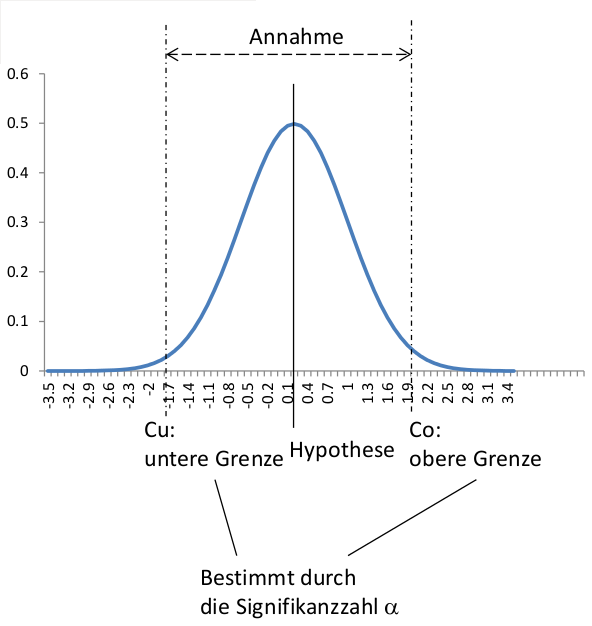
\includegraphics[scale=0.25]{images/exev_testverfahren_fehlerart_1.png}
\caption{Fehler ersten Art}
\label{fig:testverfahren:fehler1}
\end{figure}
\subsubsection{Fehler zweiter Art}
Der Fehler der zweiten Art, bedeutet eine fehlerhaftes Annehmen einer Hypothese. 
\begin{figure}[htb]
\centering
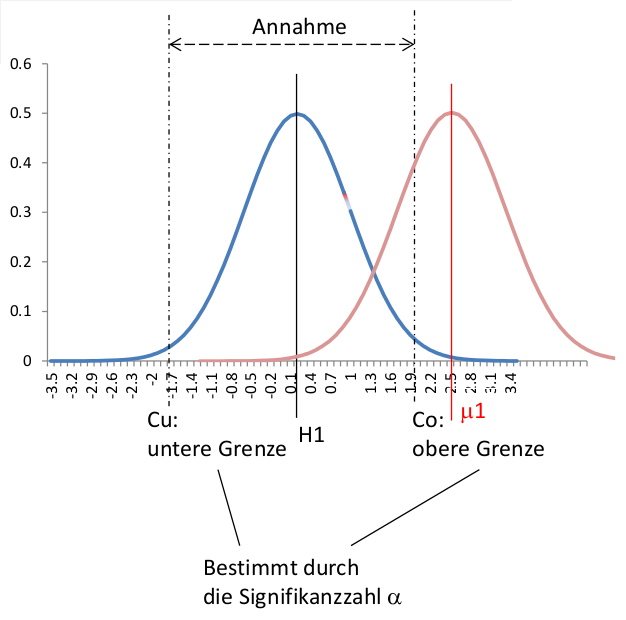
\includegraphics[scale=0.25]{images/exev_testverfahren_fehlerart_2.png}
\caption{Fehler zweiter Art}
\label{fig:testverfahren:fehler2}
\end{figure}
Beim Aufstellen einer Hypothese kann es passieren, dass diese nicht komplett der Wahrheit entspricht. Der Fehler der Hypothese und der Wahrheit wird als Fehler $\beta$ durch die Fläche von $\infty$ bis an das Ende der Annahme angegeben.
\subsubsection{Fallunterscheidungen}
Man kann unter verschiedenen Fällen unterscheiden. Unter anderem:
\begin{itemize}
\item Der/die interessierenden Parameter der Grundgesamtheit sind z.B als Erfahrungswert bekannt. Durch Stichproben soll überprüft werden, ob diese Werte noch eingehalten werden. 
\item Hypothesen basieren auf Sollwerten und Normen. Diese Werte müssen also durch Vorgaben eingehalten werden. es ist zu überprüfen, ob ein Standard eingehalten wird.
\item Hypothesen aufgrund einer Theorie oder auch auf Grund von Ergebnissen aus Simulationsläufen.
\end{itemize}
Ein statistischer Test ist eine Methoden, die eine Entscheidung ermöglichen soll. Deshalb braucht man ein bestimmtes Verfahren, um Hypothesen zu testen.
\begin{enumerate}
\item Festlegen der Grundgesamtheit und Formulieren der Nullhypothese $H_0$ und der Alternativhypothese $H_1$ (im Allgemeinen die Verneinung der Nullhypothese)
\item Festlegen der Signifikanzzahl $\alpha$, gibt die Irrtumswahrscheinlichkeit an oder das Vertrauensintervall $1-\alpha$
\item Bestimmen der Testgrösse und des Annahme und Ablehnungsbereichs. Testgrösse kann der Stichprobenmittelwert sein
\item Berechnen des Wertes der Testgrösse mit den Daten der Stichprobe und Testentscheidung
\end{enumerate}
Um Hypothesen zu beweisen, formuliert man oft eine Verneinung dieser Hypothese als Nullhypothese und versucht dann, diese durch einen statistischen Test zu wiederlegen. Dies ist Vergleichbar mit dem Indirekten Beweis der Mathematik.
\subsubsection{Parametertest}
Der Paramtertest überprüft die Hypothese über Paramter einer Grundgesamtheit.
\begin{equation}
\mu_{0} - z \frac{\sigma}{\sqrt{n}}\leq\overline{x}\leq\mu_{0}+z \frac{\sigma}{\sqrt{n}} \label{eq:parameter:1}
\end{equation}
Die Fragen die sich beim Paramtertest stellen sollten sind:
\begin{itemize}
\item Liegt eine systembedingte Störung vor?
\item Ist der angegebene Mittelwert korrekt?
\item Liegt das Ergebniss im Bereich der statistischen Schwankungsbreite (Tolleranz)?
\end{itemize}
Diese Fragen können über das Vertrauensintervall (\autoref{eq:parameter:1}) beantwortet werden.
%BEISPIEL: Folie 11
\subsubsection{Anteilswerte}
Diese können analog zu den Paramtertests angewendet werden:
\begin{enumerate}
\item Wähle die Signifikanzzahl $\alpha$ und bestimme daraus die Werte für $Z$ aus der Tabelle ($1-\alpha$)
\item Berechne die Annahmegrenzen 
\end{enumerate}
\begin{align}
c_u &= p_0 - z\displaystyle\sqrt{\frac{p_0(1-p_0)}{n}}&\quad\mbox{oder} \\
c_u &= p_0 - z\displaystyle\sqrt{\frac{p_0(1-p_0}{n}}\,\sqrt{\frac{N-n}{N-1}}&\quad\mbox{und} \\
c_0&=p_0 + z\displaystyle\sqrt{\frac{p_0(1-p_0)}{n}}&\quad\mbox{oder} \\
c_0&= p_0 + z \displaystyle\sqrt{\frac{p_0(1-p_0)}{n}}\,\sqrt{\frac{N-n}{N-1}}&
\end{align}
\begin{enumerate}
  \setcounter{enumi}{2}
  \item Man berechne den Anteil $\overline{p}=\frac{k}{n}$
  \item Fällt $\overline{p}$ in den Annahmebereich: $c_u\leq\overline{p}\leq c_0$, wird die Hypothese angenommen, sonst abgelehnt.
\end{enumerate}
%BEISPIEL Folie 15
\subsubsection{Differenztests}
Manchmal will man mit Hilfe von Stichproben untersuchen, ob  zwei Mittelwerte $\mu_1 = \mu_2$ sind, oder signifikant voneinander abweichen. Zum Beispiel ist das Ergebnis des einen (Simulations)Experiments signifikant unterschiedlich von dem anderen.  Dabei werden zwischen zwei Stichproben unterschieden
\begin{itemize}
\item Abhängige Stichproben
\subitem Diese werden in der Regel angestrebt, wenn es sonst zu Überlagerungen kommt, die das Ergebnis verzerren könnten.
\item Unabhängige Stichproben
\subitem Diese liegen dann vor, wenn zum Beispiel für ein Herstellungsprozess zwei unterschiedliche Modellvarianten untersucht werden sollen, in denen der Durchsatz untersucht werden soll.
\end{itemize}
Abhängige Stichproben erstellen:
\begin{enumerate}
\item Bilden der Nullhypothese
\begin{equation}\label{eq:differenz:nullhyp}
H_0: \mu_1 = \mu_2
\end{equation}
\item Die Differnezen der Stichprobe müssen für alle $i$ erfasst werden
\begin{equation}\label{eq:differenz:diff}
d_i = x_i - y_i
\end{equation}
\item Dann gilt die Nullhypothese $H_0$ gleich, wenn der Mittelwert von $d_i$ im Bereich von $1-\alpha$ liegt
\item Es wird die Signifikanzzahl $\alpha$ gewählt
\item Mit Hilfe der Tabelle für Normalverteilung werden die Annahmegrenzen festgelegt
\end{enumerate}
Unabhängige Stichproben erstellen:
\begin{enumerate}
\item Lege eine Signifikanzzahl $\alpha$ fest
\item Mit Hilfe der Tabelle für Normalverteilung wird der Werte $\mp Z$ festgelegt
\item Berechnung des Annahmebereichs
\footnote{Nach wie vor ist der Mittelwert gleich dem Mittelwert der Differenz. Aber jetzt muss die Varianz für jede Probe separat angenommen bzw. Geschätz werden.}
\begin{equation}
c=\mp z\sqrt{\frac{\sigma_1^2}{n_1}+\frac{\sigma_2^2}{n_2}}
\end{equation}

\item Berechnung der Mittelwerte der Stichproben $\mu_1$ und $\mu_2$
\item Man nehme die Nullhypothese aus \autoref{eq:differenz:nullhyp} an, wenn die Differenz aus \autoref{eq:differenz:diff} in den Annahmebereich fällt
\end{enumerate}
%BEISPIELE
\subsubsection{Verteilungstests}
Bisher wurden Tests behandelt, die sich auf Parameter der Grundgesamtheit beziehen. Nun soll mithilfe von Stichproben überprüft werden, ob Hypothesen über Wahrscheinlichkeitsverteilungen überprüft werden können. Verbreitete Testverfahren in den Verteilungstests sind:\footnote{Als einziger dieser Verfahren haben wir die Chi-Quadrat Verteilung behandelt}
\begin{itemize}
\item Chi-Quadrat Test (\autoref{theorie:chiquadrat})
\item Kolmogoroff-Smirnoff Test
\item Spezielle Tests, die für die Überprüfung bestimmter Verteilungen zugeschnitten sind
\end{itemize}
Die Idee des $\chi$-Quadrat Test ist, es werden die Häufigkeiten der empirische ermittelten Verteilun mit der theoretischen Verteilung verglichen. Dazu werden wieder die Differenzen der Häufigkeitswerte quadriert, normiert und aufaddiert.
\begin{align}\label{eq:testverfahren:verteilung1}
y=&\sum_i^m \frac{\left(n_i - np_i\right)^2}{np_i}\\
y=&\sum_i^m \frac{\left(h_i^e-h_i^{th}\right)^2}{h_i^{th}}
\end{align}
Geht man davon aus, dass die einzelnen Messungen wieder Normalverteilt sind, dann ist die Summe $y$ Chi-Quadrat verteilt mit $m-1$ Freiheitsgraden.\\
Um den Test zu erhalten, geht man folgendermassen vor:
\begin{enumerate}
%\setcounter{enumi}{0}
\item $H_0$: Die empirische Häufigkeit entspricht der theoretischen Häufigkeit
\item Man wähle eine Signifikanzzahl $\alpha$ und bestimme die Anzahl der Freiheitsgrade
\subitem Sind alle Parameter der Verteilungfunktion bekannt, haben wir $m-1$ Freiheitsgrade
\subitem Wenn die Parameter der Verteilungsfunktion geschätzt werden müssen, kann die Anzahl Freiheitsgrade für jeden geschätzen Parameter um eins reduziert werden.
\item Die Annahmegrenze $C_o$ wird aus der Tablle für die Chi-Quadrat Verteilung ermittelt. Die Häufigkeit sollte nicht kleiner als 5 und der Stichprobenumfang nicht grösser als 30 sein. Sonst muss man mit der YATES Korrektur arbeiten
\item Man berechnet für die vorliegenden Sithcproben den Testwert mit \autoref{eq:testverfahren:verteilung1}
\item Gilt $Y>C_0$, dann lehnt man die Hypothese $H_0$ ab, ansonsten nimmt man sie an
\end{enumerate}
%BILD folie 26
\subsubsection{Unabhängigkeitstest}
Die Unabhängigkeitstests beinhaltet die Überprüfung von eventuellen Abhängigkeiten zwischen bestimmten Zufallsvariablen. Man spricht auch von einem Chi-Quadrat Unabhängigkeitstest. Voraussetzungen dafür sind, dass die Häufigkeit grösser als 5 ist und der Stichprobenumfang grösser als 30. Dieser Test liefert eine Entscheidung ob eine Abhängigkeit besteht, jedoch keine Information oder Mass über die Stärke der Abhängigkeit (siehe \autoref{theorie:regression}). Sind diese Voraussetzungen nicht erfüllt können Korrekturen vorgenommen werden, die sogenannte YATES Korrektur. Da es jedoch auch hier keine festen Regeln gibt, und die Ergebnisse mit Vorsicht zu bewerten sind, sollten aus praktischer Sicht die Voraussetzungen erfüllt werden.
%BEISPIEL